\section{Paso 2: Asesor}

  \paragraph{}Llegados a este punto le toca el turno al asesor. Este usuario,
  debe acceder a la aplicación con el nombre de usuario y contraseña con el que
  le fue indicado en el correo electrónico de confirmación de creación de
  usuario, que le fue enviado a su cuenta de correo. La figura
  \ref{capturaPaginaInicial} muestra la página inicial de la aplicación donde se
  debe realizar este acceso.

  \subsection{Información del alumno}

  \paragraph{}Una vez el usuario ha accedido a la zona del asesor
  principal, procede a ver los alumnos a los que presta asesoría, para ello lo
  hace de la misma forma que se explicó en el capítulo \ref{verAlumnos},
  \textit{Ver alumnos}. La figura \ref{ejemploVerAlumnos} muestra la captura
  de pantalla de esta pantalla.

  \begin{figure}[!ht]
    \begin{center}
      \fbox{
      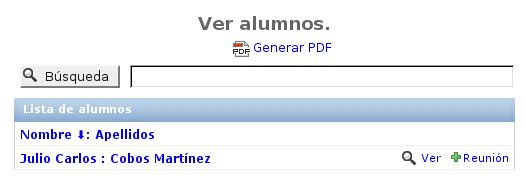
\includegraphics[scale=0.55]{5.Ejemplos_Practicos/5.4.Asesor/ver_alumnos.png}
      }
      \caption{Lista de \textit{Alumnos} de ejemplo.}
      \label{ejemploVerAlumnos}
    \end{center}
  \end{figure}

  \paragraph{}Para ver la matriculación de este alumno, pulsa sobre su nombre o
  en el icono \textit{Ver}, lo que le lleva a matriculación del alumno, que en
  nuestro caso es de tres asignaturas.

  \subsection{Creación de plantilla y preguntas}

  \paragraph{}Para crear la plantilla, el usuario asesor debe proceder de la
  misma manera que en el capítulo \ref{addPlantillaAsesor},
  \textit{Añadir plantilla de asesor}.

  \paragraph{}Para crear las preguntas, el usuario asesor debe proceder de la
  misma manera que en el capítulo \ref{addPreguntaAsesor},
  \textit{Añadir pregunta de asesor}, para cada una de las preguntas vistas en
  en capítulo \ref{enunciado}, \textit{Enunciado}.

  \paragraph{}Al final, el usuario asesor debería ver la lista con la plantilla
  y preguntas recién creadas, lista para añadir a una entrevista. La figura
  \ref{ejemploListaPreguntas} muestra esta ventana.

  \begin{figure}[!ht]
    \begin{center}
      \fbox{
      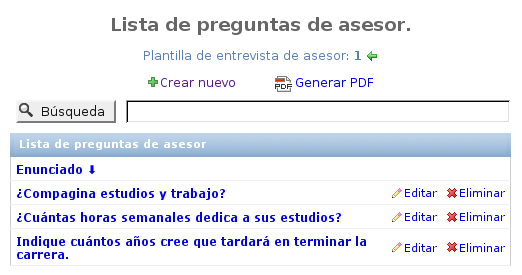
\includegraphics[scale=0.55]{5.Ejemplos_Practicos/5.4.Asesor/lista_preguntas.png}
      }
      \caption{Lista de \textit{Preguntas} de ejemplo.}
      \label{ejemploListaPreguntas}
    \end{center}
  \end{figure}

  \subsection{Creación de reunión}

  \paragraph{}Seguidamente este usuario convoca una reunión individual con el
  alumno, estableciendo las preguntas recientemente creadas, del mismo modo que
  se describió en el capítulo \ref{addReunionIndividual},
  \textit{Añadir reunión individual}. La figura \ref{ejemploReunionIndividual}
  muestra una captura de pantalla de la reunión creada.

  \begin{figure}[!ht]
    \begin{center}
      \fbox{
      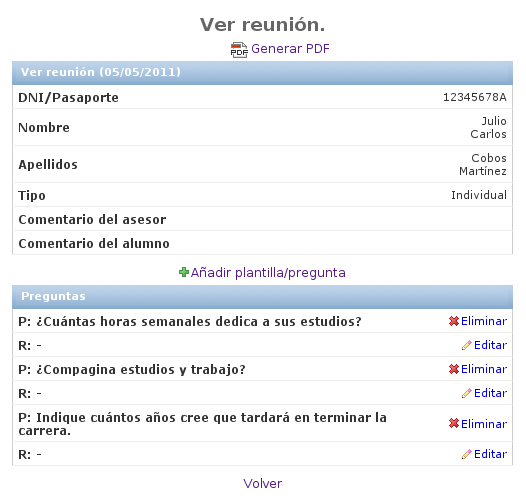
\includegraphics[scale=0.55]{5.Ejemplos_Practicos/5.4.Asesor/ver_reunion.png}
      }
      \caption{\textit{Reunión individual} de ejemplo.}
      \label{ejemploReunionIndividual}
    \end{center}
  \end{figure}
